% Standard pen-and-paper worksheet preamble.
% Compile with: xelatex -interaction=nonstopmode exercise.tex   (run twice)
\documentclass[a4paper, 14pt]{extarticle}
\usepackage[top=1in, bottom=1in, left=1in, right=1in]{geometry}
\usepackage{amsmath}
\usepackage{amssymb}
\usepackage{graphicx}
\usepackage{hyperref}
\usepackage{tcolorbox}
\usepackage{enumitem}
\usepackage{multicol}
\usepackage{adjustbox}
\usepackage{etoolbox}
\usepackage{tikz}
\usepackage{fontspec}
\usetikzlibrary{calc,decorations,patterns,arrows,decorations.pathmorphing,positioning}
\definecolor{pltblue}{HTML}{1F77B4}

% Handwriting font, resolved once into \ppfont and \ppfontname.
%
% "Pretty Neat" (xkcd-style) is the house face and is installed on almost
% nothing. Excalifont is vendored in tools/fonts/ and installed by CI, so it is
% the one face that is always present; Latin Modern is the last resort.
%
% Naming a font that is not installed is a hard error, not a fallback, which is
% why this is a chain and not a line: seven sheets used to name one outright
% and stopped building the day it was uninstalled.
\def\ppfontname{Latin Modern Roman}
\IfFontExistsTF{Pretty Neat}{\def\ppfontname{Pretty Neat}}{%
  \IfFontExistsTF{Humor Sans}{\def\ppfontname{Humor Sans}}{%
    \IfFontExistsTF{Excalifont}{\def\ppfontname{Excalifont}}{}}}
\expandafter\newfontfamily\expandafter\ppfont\expandafter{\ppfontname}
\expandafter\setmainfont\expandafter{\ppfontname}
\tikzset{every picture/.style={/utils/exec={\ppfont}}}
\AtBeginEnvironment{tabular}{\ppfont}

% xkcd-style hand-drawn line decoration.
% WARNING: applying [xkcd] to many nodes can throw "Dimension too large".
% Use it on a handful of \draw lines only, never on every node.
\makeatletter
\pgfset{
  /pgf/decoration/randomness/.initial=2,
  /pgf/decoration/wavelength/.initial=100
}
\pgfdeclaredecoration{sketch}{init}{
  \state{init}[width=0pt,next state=draw,persistent precomputation={
    \pgfmathsetmacro\pgf@lib@dec@sketch@t0
  }]{}
  \state{draw}[width=\pgfdecorationsegmentlength,
  auto corner on length=\pgfdecorationsegmentlength,
  persistent precomputation={
    \pgfmathsetmacro\pgf@lib@dec@sketch@t{mod(\pgf@lib@dec@sketch@t+pow(\pgfkeysvalueof{/pgf/decoration/randomness},rand),\pgfkeysvalueof{/pgf/decoration/wavelength})}
  }]{
    \pgfmathparse{sin(2*\pgf@lib@dec@sketch@t*pi/\pgfkeysvalueof{/pgf/decoration/wavelength} r)}
    \pgfpathlineto{\pgfqpoint{\pgfdecorationsegmentlength}{\pgfmathresult\pgfdecorationsegmentamplitude}}
  }
  \state{final}{}
}
\tikzset{xkcd/.style={decorate,decoration={sketch,segment length=0.5pt,amplitude=0.5pt}}}
\makeatother

\setlength{\parindent}{0pt}
\setlength{\parskip}{0.5em}

\begin{document}

\section*{Six Handshakes to a Stranger}

In 1967, a psychologist mailed a packet to a few hundred people in Omaha,
Nebraska. The instructions: this packet must reach a stockbroker in Boston.
You may not mail it to him directly. You may only hand it to \emph{someone you
know personally on a first-name basis}, and ask them to do the same.

{\bf Question 1}:
Write down your guess before reading on. How many hands did the packet pass
through before it arrived? \underline{\hspace{2cm}}

And write down \emph{why} you guessed that number.

\underline{\hspace{\textwidth}}

\clearpage

\section*{Part 1: The town of Ringville}

Sixteen people live in Ringville. They sit in a circle, and each person knows
only the two people sitting next to them --- nobody else.

\begin{center}
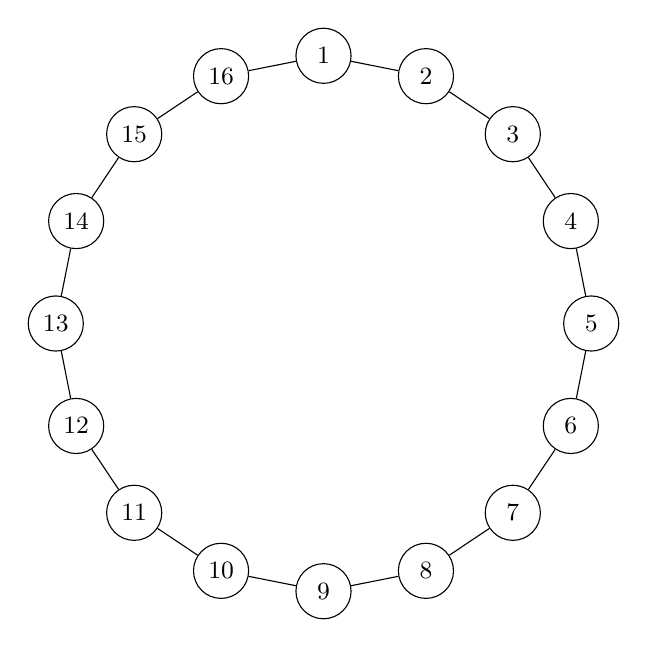
\begin{tikzpicture}[scale=1.0]
    \foreach \i in {1,...,16} {
        \node[draw, circle, inner sep=1pt, minimum size=7mm]
            (N\i) at ({90-(\i-1)*22.5}:3.4) {\small \i};
    }
    \foreach \i in {1,...,16} {
        \pgfmathtruncatemacro{\j}{mod(\i,16)+1}
        \draw (N\i) -- (N\j);
    }
\end{tikzpicture}
\end{center}

{\bf Question 2}:
Person 1 wants to get a message to person 9. Trace the shortest chain of
handshakes on the drawing. How many handshakes is it? \underline{\hspace{2cm}}

Now do this for everybody. Fill in the number of handshakes from person 1 to
each other person.

\begin{center}
\begin{tabular}{|c|p{0.7cm}|p{0.7cm}|p{0.7cm}|p{0.7cm}|p{0.7cm}|p{0.7cm}|p{0.7cm}|p{0.7cm}|}
\hline
To & 2 & 3 & 4 & 5 & 6 & 7 & 8 & 9 \\
\hline
Handshakes & & & & & & & & \\[0.5cm]
\hline
\end{tabular}

\vspace{0.3cm}

\begin{tabular}{|c|p{0.7cm}|p{0.7cm}|p{0.7cm}|p{0.7cm}|p{0.7cm}|p{0.7cm}|p{0.7cm}|}
\hline
To & 10 & 11 & 12 & 13 & 14 & 15 & 16 \\
\hline
Handshakes & & & & & & & \\[0.5cm]
\hline
\end{tabular}
\end{center}

{\bf Question 3}:
On average, how far away is a Ringville resident from person 1?
\underline{\hspace{2cm}}

And how far away is the \emph{unluckiest} pair --- the two people who need the
most handshakes of anyone in town? \underline{\hspace{2cm}}

Give these two numbers a name of your own. Which one would you quote to a
newspaper, and which one to an engineer who has to guarantee delivery?

\underline{\hspace{\textwidth}}

\clearpage

{\bf Question 4}:
Ringville grows. Now 32 people sit in the circle, still shaking hands only with
their two neighbors. You do not need to redraw anything --- just reason about it.

\begin{enumerate}
    \item The unluckiest pair in the 32-person town is \underline{\hspace{2cm}}
          handshakes apart.
    \item If the town grows to 1{,}000 people? \underline{\hspace{2cm}}
          To 8 billion? \underline{\hspace{2cm}}
    \item In one sentence: how does the worst case grow as the town grows?

    \underline{\hspace{\textwidth}}
\end{enumerate}

Ringville is a perfectly reasonable model of a village: your friends are the
people near you. But the numbers you just wrote down say that a world wired
this way could never deliver a packet from Omaha to Boston in a handful of
steps. Something must be wrong with the model.

\vspace{2em}

{\bf Question 5}:
Two people in Ringville go to college far away and each makes one distant
friend back home. Add exactly two new connections to the town: \textbf{1--9}
and \textbf{5--13}. Draw them on the circle below.

\begin{center}
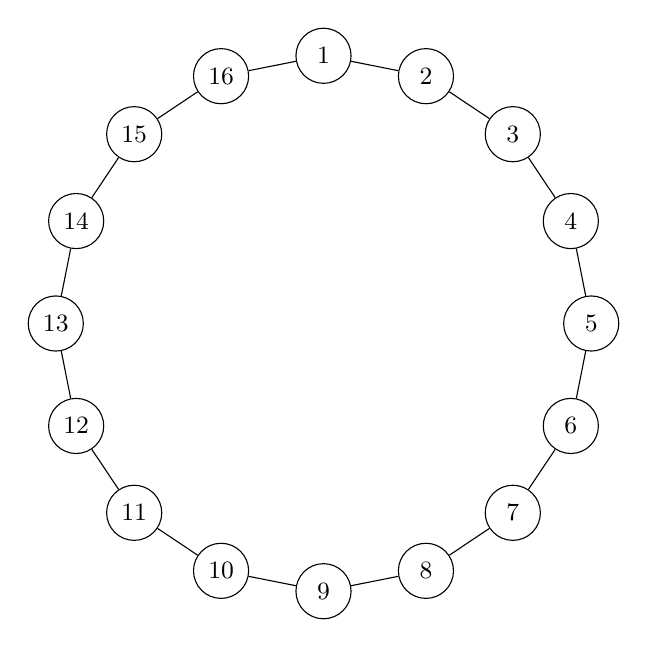
\begin{tikzpicture}[scale=1.0]
    \foreach \i in {1,...,16} {
        \node[draw, circle, inner sep=1pt, minimum size=7mm]
            (N\i) at ({90-(\i-1)*22.5}:3.4) {\small \i};
    }
    \foreach \i in {1,...,16} {
        \pgfmathtruncatemacro{\j}{mod(\i,16)+1}
        \draw (N\i) -- (N\j);
    }
\end{tikzpicture}
\end{center}

\begin{minipage}{\textwidth}
Now redo the table of Question 2 for the new town.

\begin{center}
\begin{tabular}{|c|p{0.7cm}|p{0.7cm}|p{0.7cm}|p{0.7cm}|p{0.7cm}|p{0.7cm}|p{0.7cm}|p{0.7cm}|}
\hline
To & 2 & 3 & 4 & 5 & 6 & 7 & 8 & 9 \\
\hline
Handshakes & & & & & & & & \\[0.5cm]
\hline
\end{tabular}

\vspace{0.3cm}

\begin{tabular}{|c|p{0.7cm}|p{0.7cm}|p{0.7cm}|p{0.7cm}|p{0.7cm}|p{0.7cm}|p{0.7cm}|}
\hline
To & 10 & 11 & 12 & 13 & 14 & 15 & 16 \\
\hline
Handshakes & & & & & & & \\[0.5cm]
\hline
\end{tabular}
\end{center}
\end{minipage}

\clearpage

{\bf Question 6}:
Fill in the comparison.

\begin{center}
\begin{tabular}{|l|p{3cm}|p{3cm}|}
\hline
 & Before (16 edges) & After (18 edges) \\
\hline
Average handshakes from person 1 & & \\[0.6cm]
\hline
Unluckiest pair in town & & \\[0.6cm]
\hline
\end{tabular}
\end{center}

Two connections out of eighteen were changed --- about 11\% of the town's
friendships. Was the effect on distance also about 11\%? What did those two
connections actually do?

\underline{\hspace{\textwidth}}

\vspace{4em}

{\bf Question 7}:
Predict, without computing: you add four \emph{more} distant friendships. Does
the average drop by as much again as it did the first time? Sketch a rough
curve of ``average handshakes'' against ``number of distant friendships added'',
from 0 to 16.

\begin{center}
\begin{tikzpicture}
    \draw[->] (0,0) -- (10,0) node[right] {\small distant friendships added};
    \draw[->] (0,0) -- (0,4) node[above] {\small avg handshakes};
    \foreach \x in {0,2,...,10} { \draw (\x,-0.1) -- (\x,0.1); }
\end{tikzpicture}
\end{center}

\vspace{2em}

{\bf Question 8}:
Here is the catch. You are person 1 in the rewired town, and you are holding a
packet for person 12. You cannot see the drawing --- you only know who your own
contacts are and where each of them sits in the circle. You hand the packet to
one of them, and they face the same situation.

\begin{enumerate}
    \item Play it out. Write the chain you would produce:
    $1 \rightarrow$ \underline{\hspace{6cm}}
    \item Is your chain the shortest one that exists? \underline{\hspace{2cm}}
    \item So: are ``a short chain exists'' and ``ordinary people can find a
          short chain'' the same claim? Which one did the Omaha packet
          demonstrate?

    \underline{\hspace{\textwidth}}
\end{enumerate}

\clearpage

{\bf Question 9}:
Suppose someone hands you a network of a billion people and asks for the
distance from one person to everyone else. You do not need to do it --- just
write down the procedure you would follow, in the same way you filled in the
table in Question 2. What do you do first, and what do you do at each step
after that?

\vspace{10em}

{\bf Question 10}:
Back to Omaha. Suppose every person knows 150 people, and --- pretend for a
moment --- no two of your contacts share a contact.

\begin{center}
\begin{tabular}{|c|p{2.5cm}|p{2.5cm}|p{2.5cm}|p{2.5cm}|}
\hline
Handshakes away & 1 & 2 & 3 & 4 \\
\hline
People you can reach & & & & \\[0.6cm]
\hline
\end{tabular}
\end{center}

At how many handshakes do you exceed 8 billion people? \underline{\hspace{2cm}}

Compare with the guess you wrote in Question 1. Was your guess too big or too
small --- and now that you have both Ringville and this calculation in front of
you, which assumption in this last calculation is the one you should distrust?

\underline{\hspace{\textwidth}}

\end{document}
